% =============================================================================
% 4. MODELADO PREDICTIVO
% =============================================================================
\section{Modelado predictivo}
\label{sec:modeling}

\subsection{Justificaci\'on del modelo}

Se seleccion\'o una red neuronal convolucional (CNN) con transfer learning por las razones presentadas en la Tabla~\ref{tab:justification}:

\begin{table}[H]
\centering
\caption{Justificaci\'on de decisiones de modelado.}
\label{tab:justification}
\small
\begin{tabular}{lp{4cm}}
\toprule
\textbf{Decisi\'on} & \textbf{Justificaci\'on} \\
\midrule
Deep Learning    & Im\'agenes de alta dimensionalidad ($224{\times}224$) \\
DenseNet121      & 7M par\'ametros, est\'andar en radiolog\'ia \cite{huang2017densenet} \\
TorchXRayVision  & Preentrenado en 500k+ radiograf\'ias \cite{cohen2022torchxrayvision} \\
Backbone congelado & Previene olvido catastr\'ofico \\
BCELoss+Sigmoid  & Multi-etiqueta (patolog\'ias independientes) \\
Early Stopping   & Previene sobreajuste \cite{prechelt1998early} \\
\bottomrule
\end{tabular}
\end{table}

\subsection{Arquitectura del modelo}

La arquitectura consiste en un backbone TorchXRayVision DenseNet121 congelado seguido de una cabeza clasificadora entrenada desde cero. Entrada: imagen en escala de grises $(1, 224, 224)$ normalizada a $[-1024, 1024]$. Salida: 5 probabilidades independientes $\in [0, 1]$, una por patolog\'ia (activaci\'on Sigmoid para independencia multi-etiqueta).

\subsection{Configuraci\'on de entrenamiento}

\begin{itemize}
    \item \textbf{Optimizador}: Adam ($lr = 0.001$)
    \item \textbf{Loss}: Binary Cross-Entropy (BCELoss)
    \item \textbf{M\'etrica}: MultilabelAUROC (promedio macro)
    \item \textbf{\'Epocas}: m\'aximo 20 (Early Stopping, patience = 5)
    \item \textbf{Batch size}: 32
    \item \textbf{GPU}: NVIDIA A100-SXM4-40GB
\end{itemize}

\subsection{B\'usqueda de hiperpar\'ametros}

Se realiz\'o una b\'usqueda exhaustiva (Grid Search) mediante W\&B Sweeps \cite{wandb2020} con 9 configuraciones ($3 \times 3$: learning rate $\in \{0.0001, 0.001, 0.01\}$, \'epocas $\in \{5, 10, 20\}$). La mejor configuraci\'on fue $lr = 0.001$, 5 \'epocas, con AUC = 0.8745.

\subsection{Evaluaci\'on del rendimiento}

La Tabla~\ref{tab:results-models} presenta la comparativa de rendimiento entre configuraciones:

\begin{table}[H]
\centering
\caption{Comparativa de rendimiento entre modelos.}
\label{tab:results-models}
\small
\begin{tabular}{llcc}
\toprule
\textbf{Modelo} & \textbf{Backbone} & \textbf{AUC} & \textbf{\'Epocas} \\
\midrule
TensorFlow (baseline) & ImageNet & 0.806 & 8 \\
PyTorch + ImageNet & ImageNet & 0.784 & 3 \\
\textbf{PyTorch + XRV} & \textbf{TorchXRayVision} & \textbf{0.869} & \textbf{6} \\
Sweep best & TorchXRayVision & 0.874 & 5 \\
Fine-tuning & XRV (denseblock4) & 0.868 & --- \\
\bottomrule
\end{tabular}
\end{table}

El intervalo de confianza obtenido mediante bootstrap (1000 iteraciones) fue: AUC = 0.8690 [IC 95\%: 0.8439 -- 0.8931].

\begin{figure}[H]
    \centering
    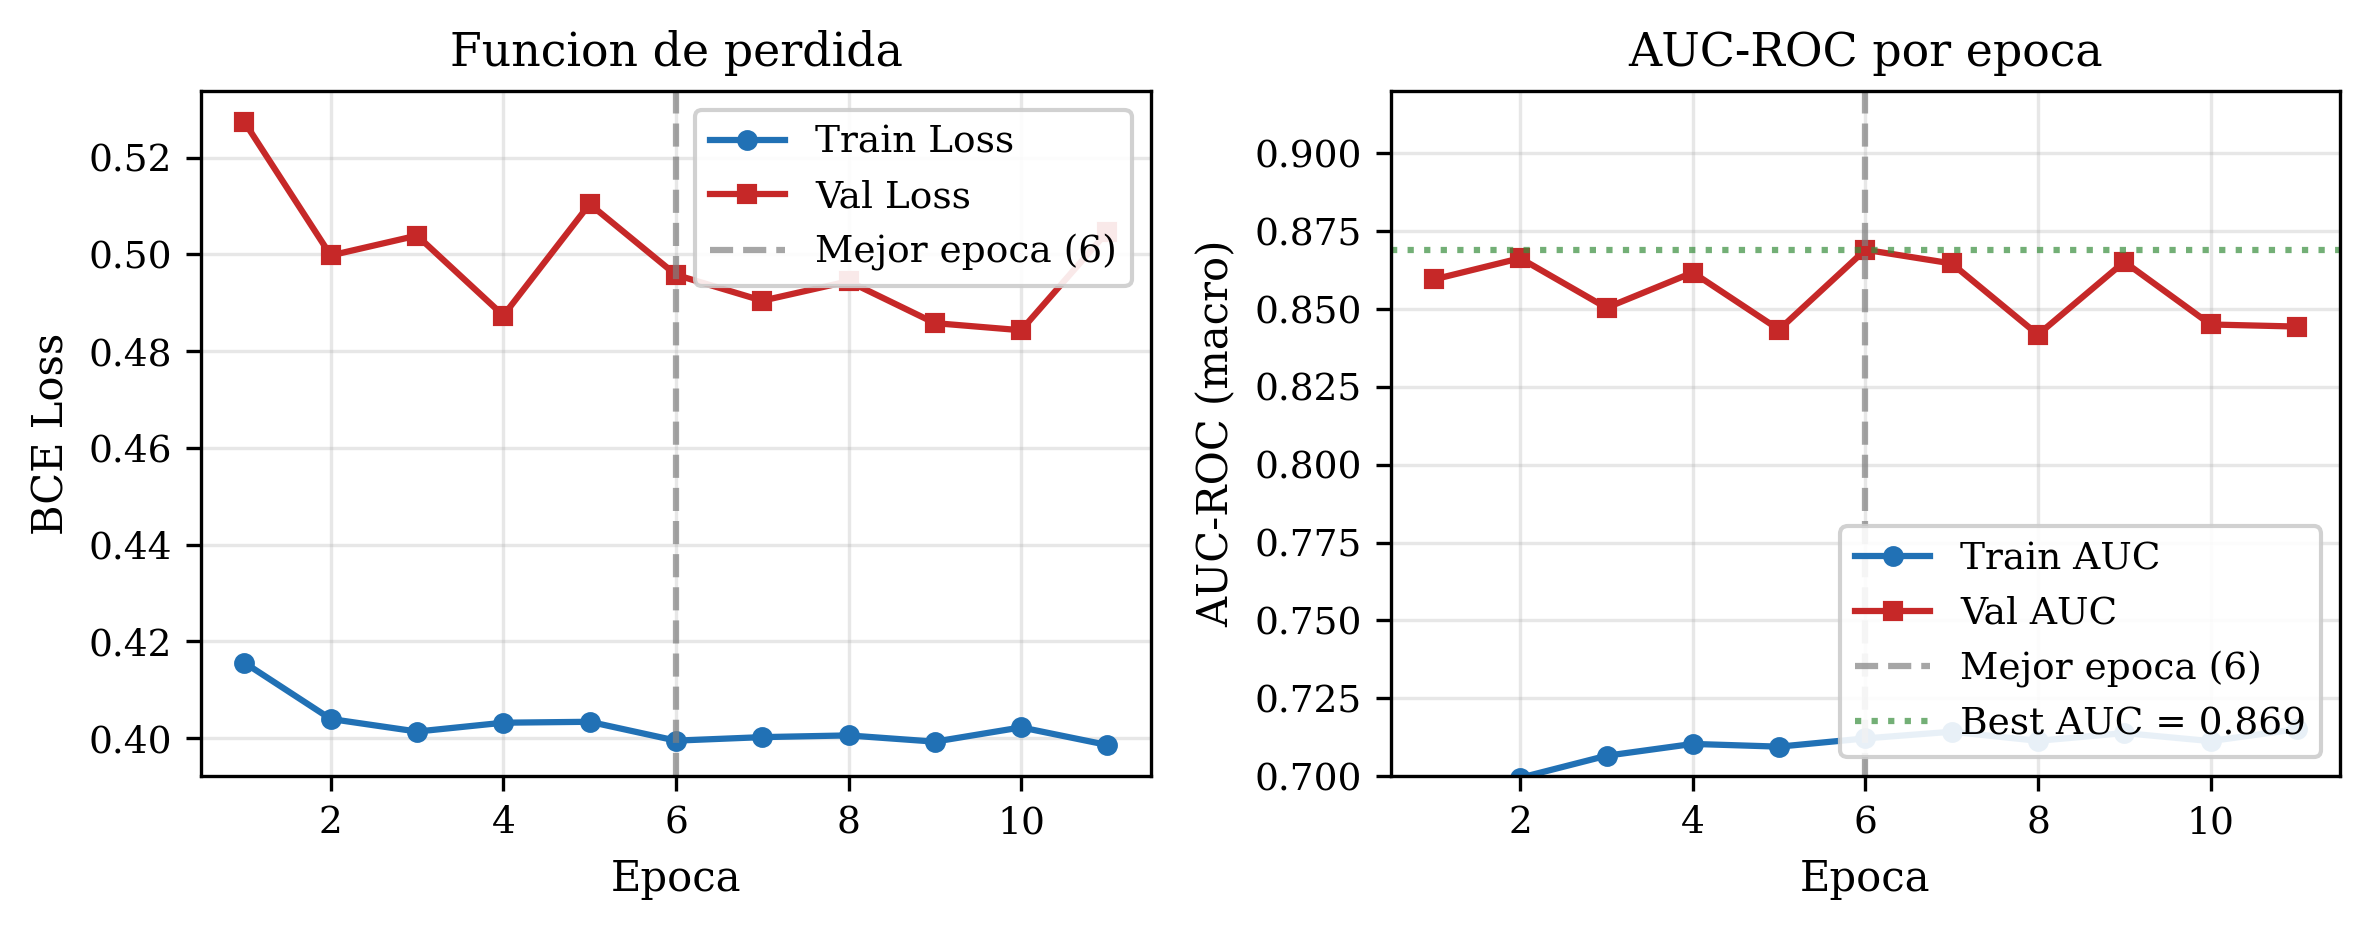
\includegraphics[width=\columnwidth]{figures/training-curves.png}
    \caption{Curvas de entrenamiento: loss y AUC por \'epoca. Early Stopping activado en \'epoca 11; mejor modelo restaurado de \'epoca 6.}
    \label{fig:training-curves}
\end{figure}

\begin{figure}[H]
    \centering
    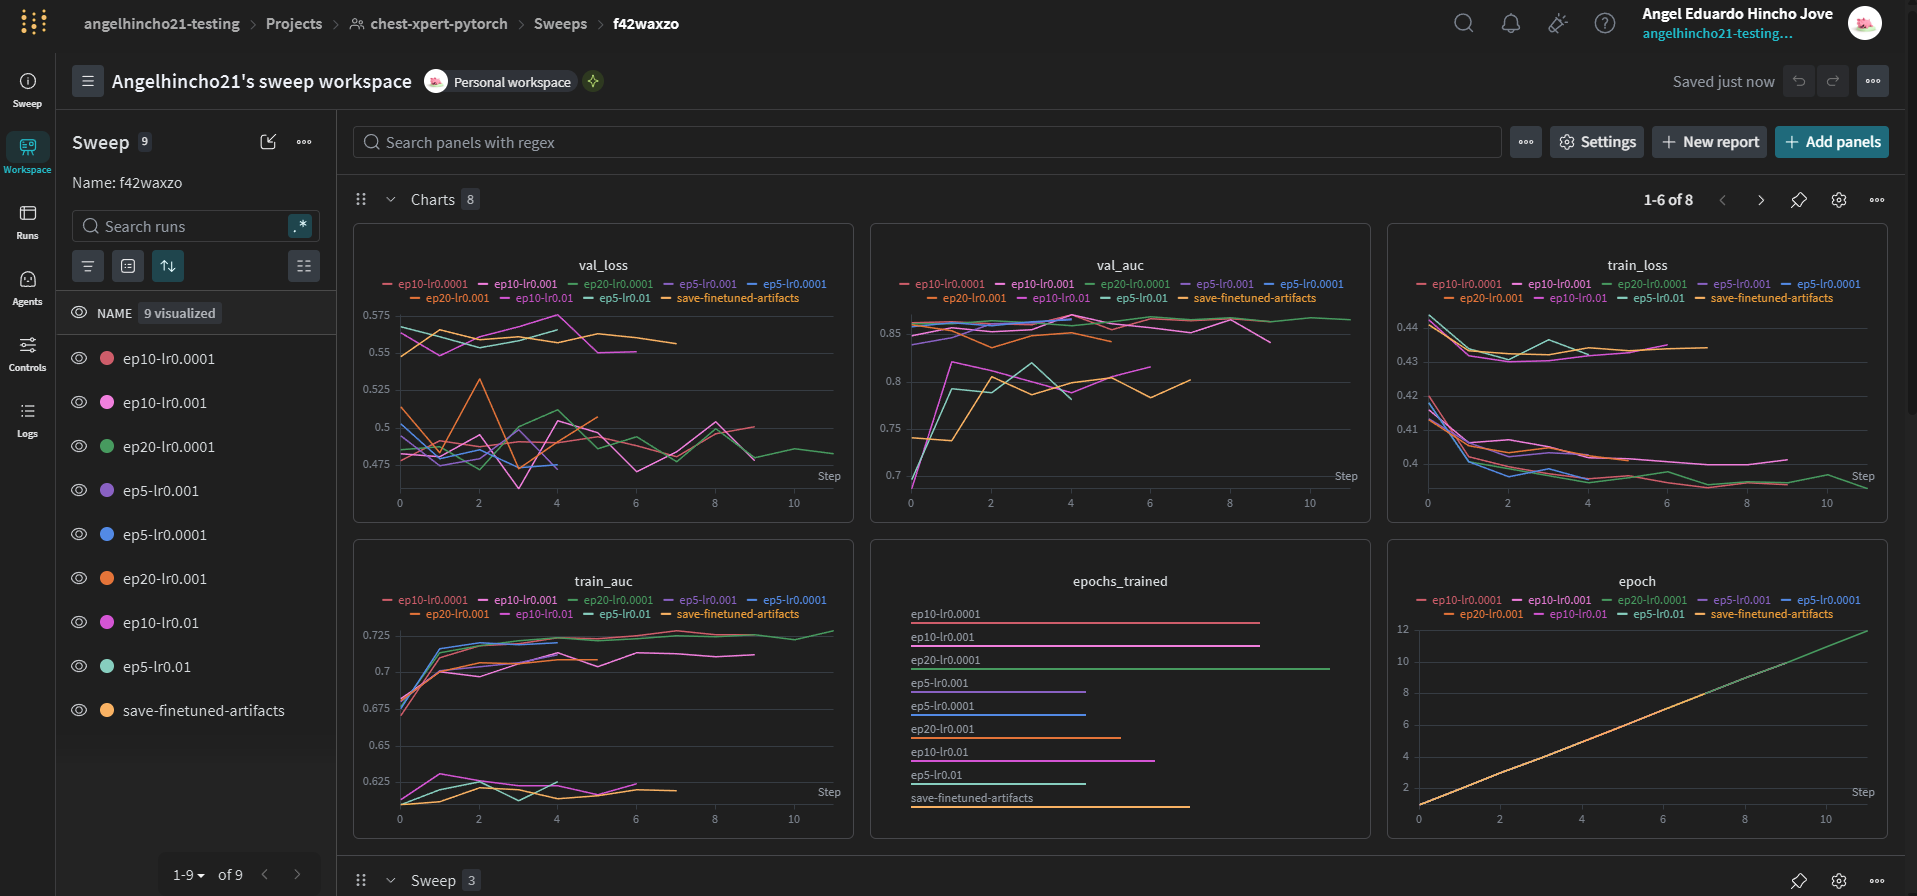
\includegraphics[width=\columnwidth]{figures/wandb-sweep-results.png}
    \caption{Resultados del W\&B Sweep: comparativa de 9 configuraciones (3 learning rates $\times$ 3 max\_epochs). Mejor: lr=0.001, 5 \'epocas.}
    \label{fig:sweep}
\end{figure}
